	% Minimal TikZ standalone example
\documentclass[tikz, border=1mm]{standalone}

\usepackage{amsmath}
\usepackage{tikz}

\usetikzlibrary{calc,angles,quotes}

\begin{document}
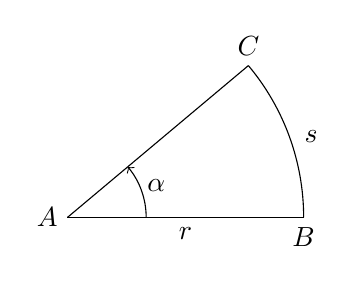
\begin{tikzpicture}[scale=1]

	% coordinates
	\coordinate (A) at (0,0);
	\coordinate (B) at (3,0);
	\coordinate (C) at ({3*cos(40)}, {3*sin(40)});

	% radius lines
	\draw (0,0) -- (3,0) node[midway, below] {$r$};
	\draw (0,0) -- ({3*cos(40)}, {3*sin(40)});

	% arc to represent the angle
	\draw (3,0) arc[start angle=0, end angle=40, radius=3]
	node[midway, right=2pt] {$s$};

	% angle marking at the center
	\pic[draw, ->, "$\alpha$", angle radius=1.0cm, angle eccentricity=1.2]
	{angle = B--A--C};


	% vertices labels
	\node[left] at (A) {$A$};
	\node[below] at (B) {$B$};
	\node[above] at (C) {$C$};

\end{tikzpicture}
\end{document}
